\documentclass[twocolumn]{article}

\def\bibsection{\section*{References}}
%\bibliographystyle{naturemag}
\usepackage[style=nature, backend=biber]{biblatex}
%\usepackage[superscript]{cite}
\bibliography{C:/Users/Dionigi/Documents/MATLAB Homework/PP6/EE189_Project/Report/refs.bib}

\usepackage{graphicx}
\usepackage{etoolbox}
\usepackage[normalem]{ulem}
\usepackage{multicol}

\newcommand{\rpm}{\raisebox{.2ex}{$\scriptstyle\pm$}}

\newcommand{\classname}{EE 189: Systems and Signals Honors}
\newcommand{\project}{-- Final Project -- \\ Heart Rate Recognition}
\newcommand{\authorname}{Brian Raymond, William Whitehead}
\newcommand{\instructor}{Prof. Fragoulis}

\usepackage{titlesec}
\titleformat{\section}
{\normalfont\large\bfseries}{\thesection}{1.5em}{}
\titleformat{\subsection}
{\normalfont\normalsize}{\thesubsection}{0.5em}{}

\begin{document}
		
	\begin{center}
		{\large \textsc{\classname \\ \project} \\ \vspace{4pt}}
		\rule[13pt]{\columnwidth}{1pt} \\ %\vspace{150pt}
		{\authorname \\ \vspace{2pt}
			Instructor: \instructor \\ \vspace{2pt}
			\today \\
		}
	\end{center}	
	
	\begin{flushleft}

		\section{Introduction}
		Given an input representing ECG signals, how does one calculate the heart rate to use for later analysis? What about with added noise obfuscating the periods? Our goal was to find the best MATLAB-based method to do this considering runtime (and therefore complexity as well). A successful algorithm in our case is one which finds the heart rate within an error of \rpm$20\%$ for $70\%$ of the given signals. \\ \vspace{-1em}
		
		\section{Approaches}
		For our purpose, we considered using a Fast Fourier Transform (FFT) approach and also a Sparse Fast Fourier Transform approach (SFFT). \\ \vspace{-2em}
		
		\hspace{2em}\subsection{FFT Method}
		After taking the FFT of the input data using MATLAB's given method, \textit{fft}, we are left with a vector containing the frequency distribution of the ECG signal. From there, we ignore all values below a certain threshold ($\frac{1}{4}$ of the maximum value) as they will likely be due to noise. On this filtered data, we then use MATLAB's \textit{findpeaks} method which returns the locations of the local maxima. The idea behind this is that within the frequency domain there will be `peaks' at the harmonic frequencies, as they are the primary components of the frequency spectrum. Therefore, once we have the harmonics, we divide the length of the input signal by the fundamental harmonic to find the period. As this has a complexity of $O(Nlog(N))$ where $N$ is the length of the input ECG signal, we also tried using a sampling rate $F_{s}=2$ to reduce the complexity to $O(\frac{N}{2}log(\frac{N}{2}))$. \\ \vspace{-2em}
		
		\hspace{2em}\subsection{SFFT Method}
		For our SFFT function, we used an algorithm which employed the process described by Hassanieh et al\cite{paperSFFT}. Given the input signal and a sparsity parameter, $k$, this algorithm outputs a vector with the estimated frequencies (harmonics). From here, the process was similar to our FFT-based method. Given the estimated harmonics, we divided the input length by the first harmonic which should be the fundamental harmonic. The total complexity is $O(klog(\frac{N}{k})log(N))$ where $N$ is the length of the input ECG signal and $k$ is the aforementioned sparsity parameter. Sampling with a rate $F_{s}$ should then reduce the complexity to $O(klog(\frac{N}{2k})log(N/2))$.  \\ \vspace{-1em}
		
		\section{Results}
		We decided to test our methods first on a vector of 10 real signals to get a general idea for its accuracy and then on 64 signals of varying noise, length, and completeness. \\ \vspace{-2em}
		
		\hspace{2em}\subsection{FFT Results} \label{ssec:resultsFFT}
		Again, both the $F_{s}=1$ and $F_{s}=2$ trials had the same results for the real signals, as they correctly identified 9 of the 10 signals with an average percent error of $2.31$. Tested on the rest of the signals, they both took the same average amount of time ($0.0009$ vs $0.0009$ seconds). The $F_{s}=1$ trial, however, found $54$ correct periods ($84.38\%$) and had an average percent error of $19.85$ compared to $46$ correct periods ($71.88\%$) and an average percent error of $41.64$ for the $F_{s}=2$ trial. \\ \vspace{-2em}
		
		\hspace{2em}\subsection{SFFT Results}  \label{ssec:resultsSFFT}
		Both the $F_{s}=1$ and $F_{s}=2$ trials had the same results for the real signals, with both correctly identifying 10 of the 10 signals with an average percent error of $2.31$. Tested on the rest of the signals, the $F_{s}=1$ trial had a slower average time ($0.0062$ vs $0.0037$ seconds) and less correct periods ($29$  or $45.31\%$ vs $31$ or $48.44\%$) against the $F_{2}=2$ trial but had a lower average percent error ($50.76$ vs $86.47$). \\ \vspace{-1em}

		 	\begin{figure*}[h]
		 	\centering
		 	\textbf{Comparison of FFT vs SFFT w/ Sampling Rate $F_{n}=1$}\par\medskip
		 	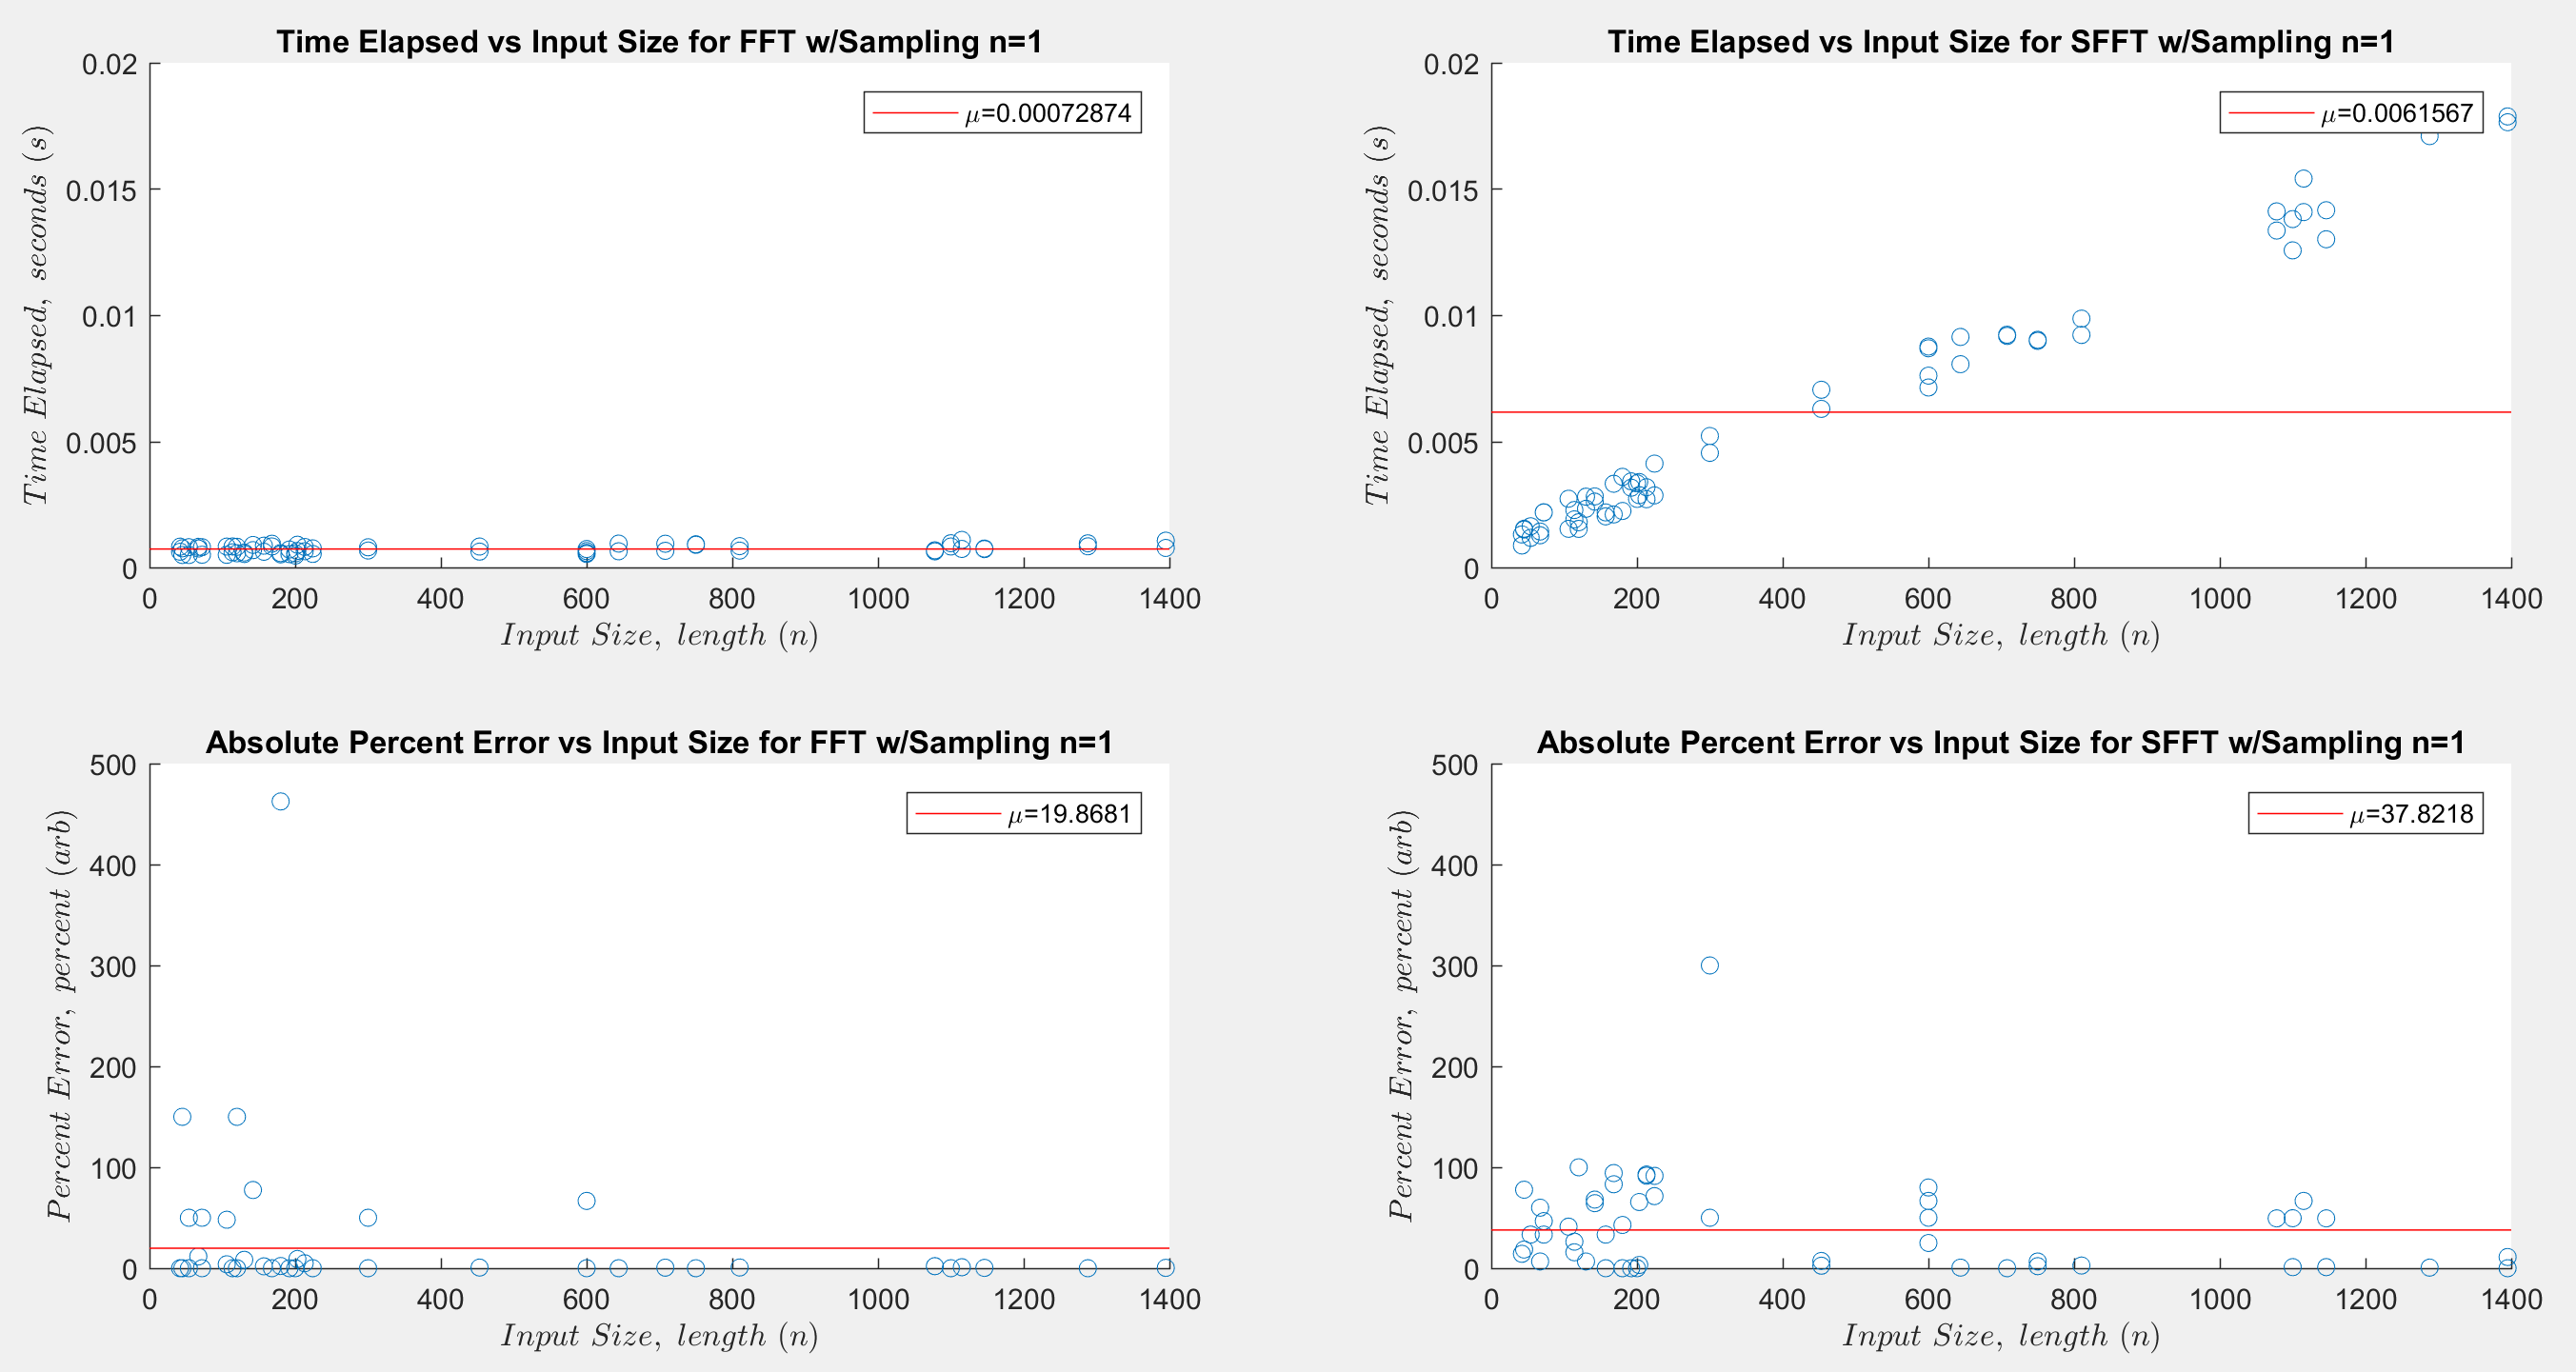
\includegraphics[width=0.9\textwidth,keepaspectratio]{FFTvsSFFT_graph.png}
		 	\caption{Comparing the FFT and SFFT approaches with a Sampling Rate of $F_{n}=1$, FFT is far superior. The FFT approach took about constant time with a mean value of $0.00072874$ seconds while the SFFT approach took a logarithmic time with a mean of $0.0061567$ seconds. Additionally, the FFT method had an average percent error of $19.8681$ while the SFFT method had an average percent error of $37.8281$.}
		 \label{fig:compareFFTandSFFT}
	 \end{figure*}
	 \hspace{2em}\subsection{FFT vs SFFT Comparison}
	 Beyond what may be restated from the previous results in subsections \ref{ssec:resultsFFT} and \ref{ssec:resultsSFFT}, looking at Figure \ref{fig:compareFFTandSFFT} gives additional insight. While the time elapsed for the FFT method was about constant with a mean value of about 0.0007 seconds, the time taken for the SFFT method increased to around two orders of magnitude larger. Meanwhile, the accuracy of the SFFT had a mean value about two times greater and was more inaccurate at both large and small input sizes compared to the FFT method. \\ \vspace{-1em}
	 \section{Conclusion}
	Based on our trials, we would choose the FFT-based method over the SFFT-based method for accurately finding the heart rates from ECG signals both quickly and efficiently. While the SFFT theoretically had a smaller complexity which was sublinear, we found it to take more time experimentally and also give less accurate results ($46.88$ percent correct) when compared to the FFT approach ($84.38$ percent correct) from our $F_{s}=1$ trials. We suspect this is due to the compiled nature of our SFFT implementation which is not as optimized as the native FFT function found in MATLAB. Were we to not use MATLAB as our environment of choice or implement both the FFT and SFFT algorithms on our own, we would instead choose to recommend an SFFT-based approach as superior.
	\printbibliography
	\end{flushleft}
	
\end{document}          
